In this chapter, we will explain the fundamentals and technologies that have been used for the experimentation. We will focus on three main aspects:
\begin{enumerate}
\item The used datasets.
\item The used libraries for the development of the code.
\item The used metrics to evaluate the obtained results.
\end{enumerate}

The idea of the experimentation part is to test and compare the frameworks that we have presented in Chapters \ref{Chapter:SimCLR} and \ref{Chapter:BYOL}. Their architectures have already been explained, and the original code for both backbones has not been done by me. 

This work will focus on testing how changing the training hyperparameters of the model affects the final results, since the original papers \cite{chen_simple_2020,grill2020bootstrap} already mention that using their structure, the results are affected by those hyperparameters, such as batch size, network depth or network width.

The implementations that have been used can be found in:
\begin{itemize}
\item SimCLR implementation: Official implementation from Google in \url{https://github.com/google-research/simclr/tree/master/tf2}

\item BYOL implementation,: Official implementation from DeepMind, found in \url{https://github.com/deepmind/deepmind-research/tree/master/byol}. 
\end{itemize}


At first, we tried to use the same library (Tensorflow) for both frameworks. However, finally it was decided that using the official implementation for BYOL, which was coded using \lstinline{Jax} was better, since some pre-sets of this implementation were useful for our case study. Also, the idea is to make use of \emph{Tensorboard}, a Tensorflow utility that helps with visualization and graph generation of the training and final results that can be used with both Jax and Tensorflow.

\section{Objectives of the experiments}

In the most ideal scenario, the main goal of our experiments should be to try to reproduce the results that the original papers have obtained and check if, under the conditions that are set, we obtain the same (or at least similar) results.

However, while carefully studying the frameworks proposed, we found that their results were obtained using the following computational resources:
\begin{itemize}
\item SimCLR's results were obtained using $128$ TPU v3 cores in around $1.5$ hours of training, using a batch size of $4096$.
\item BYOL's results were obtained using $512$ Cloud TPU v3 cores in around $8$ hours using the same batch size used in SimCLR experiments.
\end{itemize}

Approximately, the price of a single Cloud TPU V3 is $8.80\$$ per hour. If we wanted to use $128$ TPUs, it would cost a total of $\sim 1126 \$$  per hour of execution. We can not afford this pricing. 

Because of this, we decided to set a different main goal of our experiments. Our goal will be to research what results can we obtain using limited resources. Using a single GPU for each experiment, we will investigate how the hyperparameters affect to the final results in a dataset where the training times allow us to realize multiple training of the models.


\section{Language, hardware and basic libraries}

The chosen language for this project was \lstinline{Python}. There were other possibilities, such as \lstinline{R}. However, since the majority of machine learning projects are developed in \lstinline{Python}, our choice was easy.

When running training experiments in DL, the used hardware is one of the most determining factors for the results obtained by the models. There are many reasons for this, such as the time spent on the training a model or the amount of  data that we can fit in the GPU's (which will be our case) or TPU's memory.

For the experiments of this project, the DECSAI\footnotemark department of the University of Granada generously provided us access to a server that has a few NVIDIA GeForce RTX 3090. This model of GPU is one of the best in the market, having a \emph{compute capability} of $8.6/10$, rated by the NVIDIA company. IT also has a memory of $24GB$, which allows us to experiment with relatively large batch sizes using a single GPU and not having to parallelize the experiment.

%------------- Footnotemark
\footnotetext{The DECSAI's website is \url{https://decsai.ugr.es/}.}
%----------------------


To be able to use this GPUs in our experiments, three basic libraries have to be installed in the server:
\begin{enumerate}
\item \lstinline{tensorflow-gpu}. This is a variant of the \lstinline{tensorflow} library that was developed for using GPUs while using tensorflow.
\item \lstinline{Jax}, a library used to automatically differentiate native \lstinline{Python} and \lstinline{NumPy} functions.
\item \lstinline{CUDA 11.4}. CUDA is a parallel computing platform and API created by NVIDIA which allows to use a CUDA-enabled GPU for general purpose processing. In other words, CUDA is needed to be able to use the GPU in our \lstinline{python} scripts.
\end{enumerate}

These two libraries, along with other packages that are needed for creating graphics (\lstinline{Matplotlib,Seaborn}) or computing metrics (\lstinline{sklearn}) are installed using a \lstinline{Conda} environment in our server's user.


\section{The datasets}

\subsection{CIFAR10}

The computational resources that we have for the experiment are limited. Due to this, we must fix a dataset that, having enough and representative examples, allows us to achieve feasible training time and successful results.

One of the ever most used dataset, which was also used in both SimCLR and BYOL papers, is CIFAR10 \citep{krizhevsky_learning_nodate}. This dataset will be used to test the overall performance of our representation learning methods.

CIFAR10 contains $60.000$ images divided in $10$ classes, where each class contains $10.000$ images. The size of the images is $32\times 32\times 3$, so the size of the images is not very large. This helps us to have faster trainings.

\begin{figure}[H]
    \centering 
    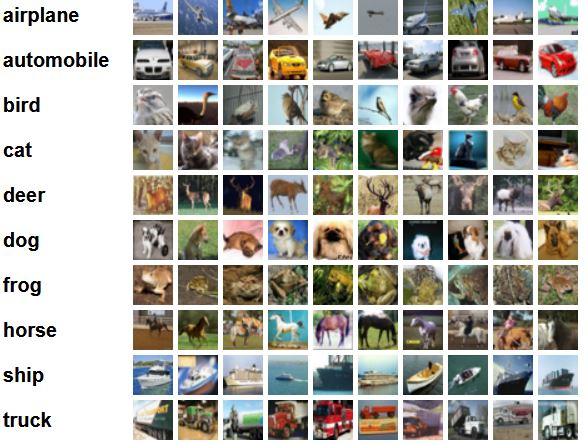
\includegraphics[scale=0.8]{CIFAR10}
    \caption{Ten examples of each class in the CIFAR10 dataset. }
\end{figure}
This dataset has $50.000$ samples for training and $10.000$ for test. The test batch contains the same number of examples of each of the $10.000$ classes in the dataset, that is, it contains $1.000$ examples of each class. 

It is important to remark that the classes are \emph{completely mutually exclusive}. That means that there is no overlap between the classes even if they have similar images, such as \emph{Cars} and \emph{Truck}, which are two of the classes of the dataset.

\subsection{Imagenette}

When we reached the part where we tried to reproduce the experiments of the BYOL framework, we discovered that the time for a single \emph{pretraining} took almost a whole day to train for $100$ epochs. Because of this, we decided to look for a solution that could make our trainings faster.

In the repository of the implementation, we found that the model could also be trained on \emph{Imagenette}. This dataset is a subset of $10$ easily classified classes from \lstinline{Imagenet} \citep{russakovsky2015imagenet}, one of the biggest and most commonly used datasets. This subset can be obtained in different image sizes depending on our purposes: full size download, $320$ px or $160$ px. We use the $160$ px version, consisting in approximately $9.000$ images for train and $4.000$ images for test.

Since the classes are easily classifiable, this dataset helps the project to test the frameworks in a friendly environment, similar to what CIFAR10 offers us, but using different classes.



\section{Tensorflow}



Tensorflow\footnotemark is an open source library for developing machine learning frameworks.  

\begin{wrapfigure}{r}{5cm}
    \caption{Tensorflow logo.}
    
\includegraphics[scale=0.2]{tf-logo}
\end{wrapfigure}

%------------- Footnotemark
\footnotetext{Tensorflow documentation can be found at \url{https://www.tensorflow.org/}.}
%----------------------



It can be used for many tasks, but it focuses on training and inference of deep neural networks. It is used for both research and production at \emph{Google}, since it was also developed by the \emph{Google Brain} team for internal use. However, it was later released as open source.

The creation of new models is very simple, offering multiple abstraction levels. This is why it is suitable for our experiments. Also, the code is most of the times easily understandable.

There are a few ways to define a NN or a framework using tensorflow. The most common one is defining a sequential model using \lstinline{Keras}, a tensorflow API that defines layers of a neural network and helps with the implementation of simple NN structures.% Let us see how to implement a very simple example of a NN with three \emph{Dense} layers: 

%\begin{minted}[mathescape,linenos]{python}
%model = keras.Sequential(
%    [
%        layers.Dense(2, activation="relu", name="layer1"),
%        layers.Dense(3, activation="relu", name="layer2"),
%        layers.Dense(4, name="layer3"),
%    ]
%)
%\end{minted}

Another way of creating models using tensorflow is by defining a single step of training using \lstinline{tf.GradientTape()} and then executing the single step multiple times in a loop. Using GradientTape , tensorflow performs automatic differentiation, which is needed for the minimization process. Let us see the simplest example, consider the function $f(x) = x^2$, and imagine that we want to obtain $f'(3)$. We can obtain it using \lstinline{tf.GradientTape()} as follows:

\begin{minted}[mathescape,linenos]{python}
x = tf.constant(3.0)
with tf.GradientTape() as g:
  g.watch(x)
  y = x * x
dy_dx = g.gradient(y, x)
\end{minted}

In our case, the gradient is obtained and the applied to the optimizer by using:

\begin{minted}[mathescape,linenos]{python}
with tf.GradientTape() as tape:
    grads = tape.gradient(loss, model.trainable_variables)
    optimizer.apply_gradients(zip(grads, model.trainable_variables))
\end{minted}


\subsection{Tensorboard}

Tensorboard is a Tensorflow's visualization kit. It provides the visualization and tooling needed for machine learning experimentation. Among its more important utilities, we can find:
\begin{itemize}
\item Tracking and visualizing metrics (such as loss, accuracy, entropy) not only during the training but also when the training time has ended.

\item Visualizing the model graph: ops and layers.

\item Visualizing histograms of weights, biases and how tensors change during the training.

\item Projecting high-dimensional data to a lower dimensional space.

\item Displaying images,text and audio data.
\end{itemize}

Also, it is very easy to integrate with tensorflow.  Actually, in most of the cases it is as simple as adding the following \emph{callback} when we fit the model:

\begin{minted}[mathescape,linenos]{python}
    tensorboard_callback = tf.keras.callbacks.TensorBoard
                        (log_dir=log_dir, histogram_freq=1)
    model.fit(x=x_train, y=y_train, 
              epochs=5, 
              validation_data=(x_test, y_test),
              # The added callback produces the magic! 
              callbacks=[tensorboard_callback])  
\end{minted}

In our case, there are some differences, since we are not using the standard \lstinline{fit} function to train our models. Because of this, we have to log the information that we have obtained in each step. To do this, we can use the \lstinline{metrics} python package to group them (as it is done in the SimCLR code), or we can just directly save the information creating a \emph{file writer} and writing the desired variables on this file. We do this in the modification that we have done to BYOL's original code as follows:

\begin{minted}[mathescape,linenos]{python}
train_summary_writer = tf.summary.create_file_writer(args.log_dir)
with train_summary_writer.as_default():
    tf.summary.scalar('top_1_acc',float(acc),step=epoch)
    tf.summary.scalar('top_5_acc',float(top_5_acc),step=epoch)
    tf.summary.scalar('loss', float(losses[-1]), step=epoch)
\end{minted}


\section{Metrics}

As we have seen, firstly, our models create a representation of the input image and then this representation is evaluated using a supervised linear head. This is the most interesting part, since we can see if the representation obtained was really useful for the classification task. We need to present the measures that we will use to measure how good the representations that we are producing are.



\begin{notation}
We will address the \emph{true positives} (the positive samples of a class classified correctly) as $TP$, the \emph{true negatives} (the negative samples classified correctly) as $TN$, the \emph{false positives} (the negative samples classified as positive ones, which is a mistake of our model) as $FP$ and the false negatives (the positive samples classified incorrectly as negative samples) as $FN$.
\end{notation}

Using this notation, the main measure that we will be using is the \emph{Accuracy}, which we know that can be expressed as follows:
\[
\operatorname{Accuracy} = \frac{TP + TN}{TP + TN + FP + FN}  .  
\] 

Accuracy is a classic measure for classification models. It measures the percentage of correct labels that our models has obtained for the representation that has been introduced to the linear head as input. In our case, we will be distinguishing two cases of accuracy:
measures that we will be using are the following:

\begin{enumerate}
\item \emph{Top1} accuracy, which is the ordinary accuracy.
\item \emph{Top5} accuracy, which measures if any of the 5 highest probability answers matches the true label. This is interesting because it tells us whether the model, if it did not classify an input correctly, it was close to doing it.
\end{enumerate}




